\begin{figure*}
  \vspace{-1.5em}
  \centering
  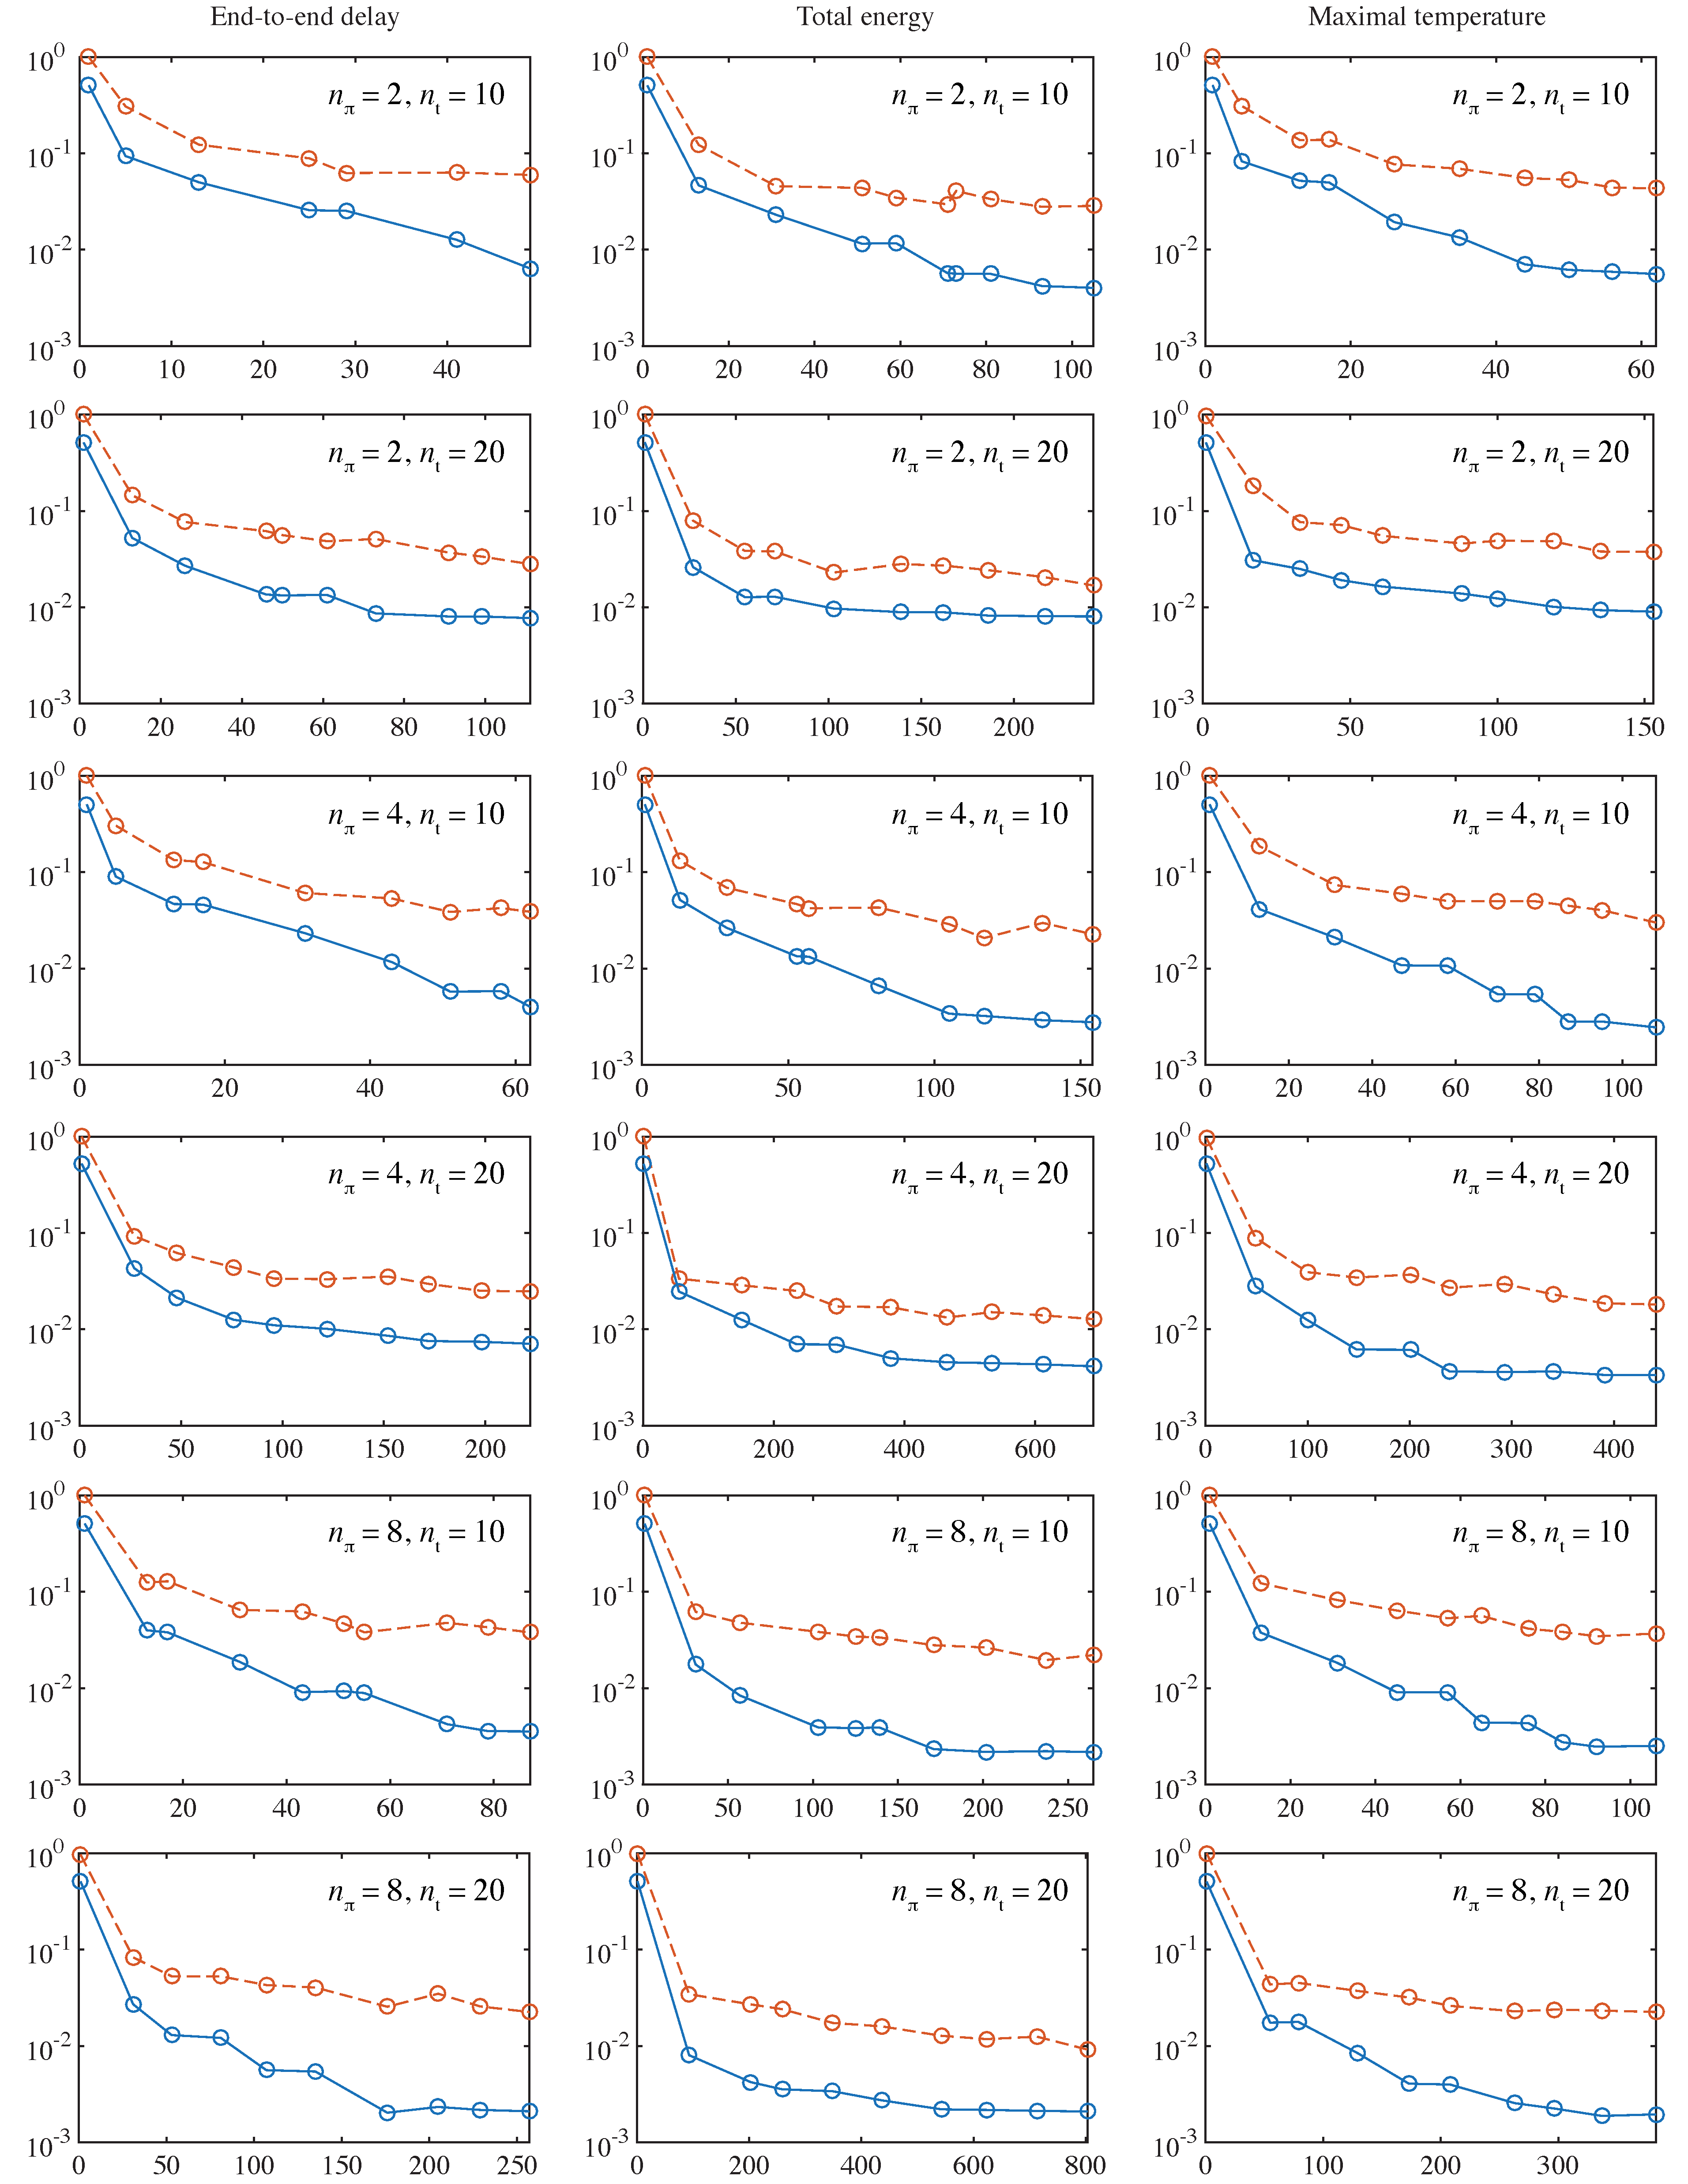
\includegraphics[width=1.0\textwidth]{include/assets/figures/results.pdf}
  \vspace{-1.5em}
  \caption{
    Experimental results. There are considered 3 platform sizes, 2 application
    sizes, and 3 quantities. The columns correspond to the three quantities: the
    end-to-end delay (left), total energy (middle), and maximum temperature
    (right). The rows alternate between the two application sizes: 10 (odd) and
    20 (even) tasks. The three pairs of rows correspond to the three platform
    sizes: 2 (top), 4 (middle), and 8 (bottom) processing elements. The
    horizontal axes show the number of points, and the vertical ones the error
    on a logarithmic scale. The solid lines correspond to our technique, and the
    dashed ones to direct sampling.
  }
  \flab{results}
\end{figure*}

The results of all 18 uncertainty-quantification problems are given in
\fref{results} as a 6-by-3 grid of plots, one plot per problem. The three
columns correspond to the three quantities of interest: the end-to-end delay
(left), total energy (middle), and maximum temperature (right). The three pairs
of rows correspond to the three platform sizes: 2 (top), 4 (middle), and 8
(bottom) processing elements. The rows alternate between the two application
sizes: 10 (odd) and 20 (even) tasks.

The horizontal axis of each plot shows the number of points, that is,
evaluations of the quantity of interest $\g$, and the vertical one shows the
\up{KS} statistic on a logarithmic scale. Each plot has two lines. The solid
line represents our technique. The circles on this line correspond to the steps
of the interpolation process given in \eref{approximation}. They show how the
\up{KS} statistic computed with respect to the reference solution changes as the
interpolation process takes steps (and increases the number of collocation
nodes) until the stopping condition is satisfied (\sref{adaptivity}). Note that
only a subset of the actual steps is displayed in order to make the figure
legible. Synchronously with the solid line (that is, for the same numbers of
$\g$'s evaluations), the dashed line shows the error of direct sampling, which,
as before, is computed with respect to the reference solution.

Let us first walk through a particular problem in \fref{results}. Consider, for
instance, the one labeled with $\bigstar$. It can be seen that, at the very
beginning, our solution and the solution of direct sampling are poor. The
\up{KS} statistic tells us that there are substantial mismatches between the
estimates and the reference solution. However, as the interpolant is being
adaptively refined, our error decreases rapidly, and, by the end of the
interpolation process, our solution becomes approximately one order of magnitude
more accurate than the one of na\"{i}ve sampling.

Studying \fref{results}, one can make a number of observations. First and
foremost, our interpolation-powered approach (solid lines) to probabilistic
analysis outperforms direct sampling (dashed lines) in all the cases. This means
that, given a fixed budget of the computation time---the probability
distributions delivered by our framework are much closer to the true ones than
those delivered by sampling $\g$ directly, despite the fact that the latter
relies on Sobol sequences, which are a sophisticated sampling strategy. Since
direct sampling methods try to cover the probability space impartially,
\fref{results} is a salient illustration of the difference between being
adaptive and nonadaptive.

It can also be seen in \fref{results} that, as the number of evaluations
increases, the solutions computed by our technique approach the exact ones. The
error of our framework decreases generally steeper than the one of direct
sampling. The decrease, however, tends to plateau toward the end of the
interpolation process (when the stopping condition is satisfied). This behavior
can be explained by the following two reasons. First, the algorithm has been
instructed to satiate certain accuracy requirements ($\aerror$, $\rerror$, and
$\serror$), and it reasonably does not do more than what has been requested.
Second, since the model-order reduction mechanism is enabled in the case of
interpolation, the quantity being interpolated is not $\g$, strictly speaking;
it is a lower-dimensional representation of $\g$, which already implies an
information loss. Therefore, there is a limit on the accuracy that can be
achieved, which depends on the amount of reduction applied. However, model-order
reduction is a good, recommended practice since it circumvents unnecessary
complexity and, thereby, makes uncertainty-quantification problems more
tractable.

The message of the above observations is that the designer of an electronic
system can benefit substantially in terms of accuracy per computation time by
switching from direct sampling to the proposed technique. If the designer's
current workhorse is the classical \up{MC} sampling, the switch might lead to
even more dramatic savings than those shown in \fref{results}. Needless to
mention that the gain is especially prominent in situations where the analysis
needs to be performed many times such as when it resides in a design-space
exploration loop.

\begin{remark}
The wall-clock time taken by the experiments is not reported in this paper
because this time is irrelevant: since the evaluation of $\g$ is time consuming
(see \sref{problem}), the number of $\g$'s evaluations is the most apposite
expense indicator. For the curious reader, however, let us give an example by
considering the problem labeled with $\clubsuit$ in \fref{results}. Obtaining a
reference solution with $10^5$ simulations in parallel on 16 processors took us
around two hours. Constructing an interpolant with 383 collocation nodes took
around 30 seconds (this is also the time of direct sampling with 383 simulations
of $\g$). Evaluating the interpolant $10^5$ times took less than a second. The
relative computation cost of sampling an interpolant readily diminishes as the
complexity of $\g$ increases; contrast it with direct sampling, whose cost grows
proportional to $\g$'s evaluation time.
\end{remark}
